\documentclass[a4paper,11pt,fleqn]{article}
\usepackage{podes-template}

%pacotes adicionais
\usepackage[linesnumbered, algoruled, vlined, portuguese]{algorithm2e}
\usepackage{listings}
\lstset
{ %Formatting for code in appendix
	language=Python,
	numbers=left,
	stepnumber=1,
	showstringspaces=false,
	tabsize=1,
	breaklines=true,
	breakatwhitespace=false,
}

%%%%%%%%%%%%%%%%%%%%%%%%%%%%%%%%%%% %%%%%%%%%%%%%%%%%%%%%%%%%%%%%%%%%%%%%%%


%título do artigo
\title{Desenvolvendo Resolvedores de Programação Linear Inteira Mista em Python usando o pacote Python-MIP$^1$} 

%define os autores
\author{
 \name{Haroldo G. Santos\authortag{a}\corresponding{haroldo@ufop.edu.br}}, 
 \name{Túlio A.M. Toffolo\authortag{a}} \\
 \authortag{a}
 \institute{Instituto de Ciências Exatas e Biológicas, Departamento de Computação\\ Universidade Federal de Ouro Preto, Ouro Preto, MG, Brasil}
}

\authorrunning{Santos \& Toffolo}


\begin{document}


\maketitle


\begin{resumo}
O pacote Python MIP oferece ferramentas para a modelagem e resolução de Problemas de Programação Inteira Mista em Python. Além de uma linguagem de modelagem de alto nível, o pacote permite o desenvolvimento de resolvedores avançados, habilitando comunicação bidirecional com o resolvedor durante o processo de busca. Neste tutorial desenvolveremos resolvedores de Programação Linear Inteira Mista para o Problema do Caixeiro Viajante. Iniciando com um resolvedor simples baseado em uma formulação compacta iremos evoluir para um resolvedor que combina heurísticas, planos de corte e estratégias de ramificação para a resolução eficaz de problemas de grande porte.

\end{resumo}

\begin{palavras}
Primeira, Segunda, Terceira, Quarta.
\end{palavras}

\begin{abstract}
This document presents the format for full papers to be published in the journal Pesquisa Operacional para o Desenvolvimento. The Abstract must not exceed 150 words.
\end{abstract}

\begin{keywords}
First keyword, Second keyword, Third keyword, Last keyword. 
\end{keywords}


\newpage
\thispagestyle{defaultPage}

Python-MIP é um pacote para modelagem e resolução de Problemas de
Programação Linear Inteira Mista (PLIM)\cite{Wolsey1998} em Python.
O projeto do pacote foi feito com o objetivo de desenvolver uma ferramenta
que atendesse os seguintes requisitos:
\begin{enumerate}
	\item clareza de código e modelagem de alto nível
	\item alto desempenho
	\item extensibilidade e configurabilidade
\end{enumerate}
Tradicionalmente, os objetivos 1 e 2 foram considerados conflitantes.
Até recentemente, as opções mais recomendada para os interessados
em 1 eram linguagens algébricas de alto nível como AMPL\cite{Fourer1987}.
A obtenção de desempenho máximo costumava requerer o uso de linguagens
de mais baixo nível como C\cite{Johnson1991a}. Resolvedores estado-da-arte
como o CPLEX\cite{Bixby2002} foram escritos nessa linguagem. Desse
modo, a biblioteca completa de funções estava originalmente somente
disponível somente nela. Recentemente, soluções como JuMP\cite{Dunning2015}
demonstraram que os objetivos 1 e 2 não são necessariamente conflitantes:
linguagens de alto nível como Julia juntamente com compiladores \emph{just-in-time}
permitem o desenvolvimento rápido de resolvedores que apresentam alto
desempenho. O objetivo do projeto Python-MIP é o desenvolvimento de
um pacote de Programação Linear Inteira Mista para a linguagem Python
que atenda plenamente os requisitos 1-3.

Pesquisas recentes mostram que Python está se tornando a linguagem
mais popular da atualidade\cite{pythonEconomist2018}. O projeto Python-MIP
foi primariamente inspirado em dois projetos de código aberto para
programação linear inteira em Python. O primeiro é o PuLP\cite{Mitchell2009},
que oferece uma linguagem de modelagem de alto nível e interface para
vários resolvedores. Recursos que requerem uma integração maior com
o resolvedor, como geração dinâmica de planos de cortes, não estão
disponíveis neste pacote. O pacote CyLP, por outro lado, suporta geração
dinâmica de planos de corte mas não oferece uma linguagem de modelagem
de alto nível\cite{Towhidi2016} e somente suporta o resolvedor COIN-OR
CBC\cite{Forrest2005}. O pacote Python-MIP foi criado com o objetivo
de prover a funcionalidade dos dois pacotes com máximo desempenho.
A escrita de um um novo pacote de programação linear inteira em Python
também permite que recursos relativamente novos da linguagem, como
a tipagem estática e a comunicação direta com bibliotecas nativas
(Python CFFI) sejam utilizados extensivamente no código.

Neste tutorial desenvolveremos versões sucessivamente mais sofisticadas
de um resolvedor para o clássico problema do caixeiro viajante no
pacote Python-MIP.

\section{Aplicação: Problema do Caixeiro Viajante}

O problema do caixeiro viajante consiste em: dada uma malha viária
e um conjunto de pontos que devem ser visitados, encontrar uma rota
de distância mínima que percorra todos os pontos percorrendo-os exatamente
uma vez. Formalmente, temos como dados de entrada um grafo direcionado
$G=(V,A)$ com distâncias associadas aos arcos:
\begin{description}
	\item [{$V$}] conjunto de vértices numerados sequencialmente a partir
	de 1
	\item [{$A$}] conjunto de arestas
	\item [{$d_{(i,j)}$}] distância do arco $a=(i,j)\in A$
\end{description}
Em todas as formulações que serão apresentadas, utilizaremos as seguintes
variáveis binárias de decisão que representam a escolha dos arcos
que compõe a rota:

\[
x_{(i,j)}=\begin{cases}
1 & \textrm{se o arco }(i,j)\textrm{ foi escolhido para a rota}\\
0 & \textrm{caso contrário}
\end{cases}
\]

Como exemplo, considere o grafo de distâncias das Figura \ref{figG}:

\begin{figure}
	\begin{centering}
		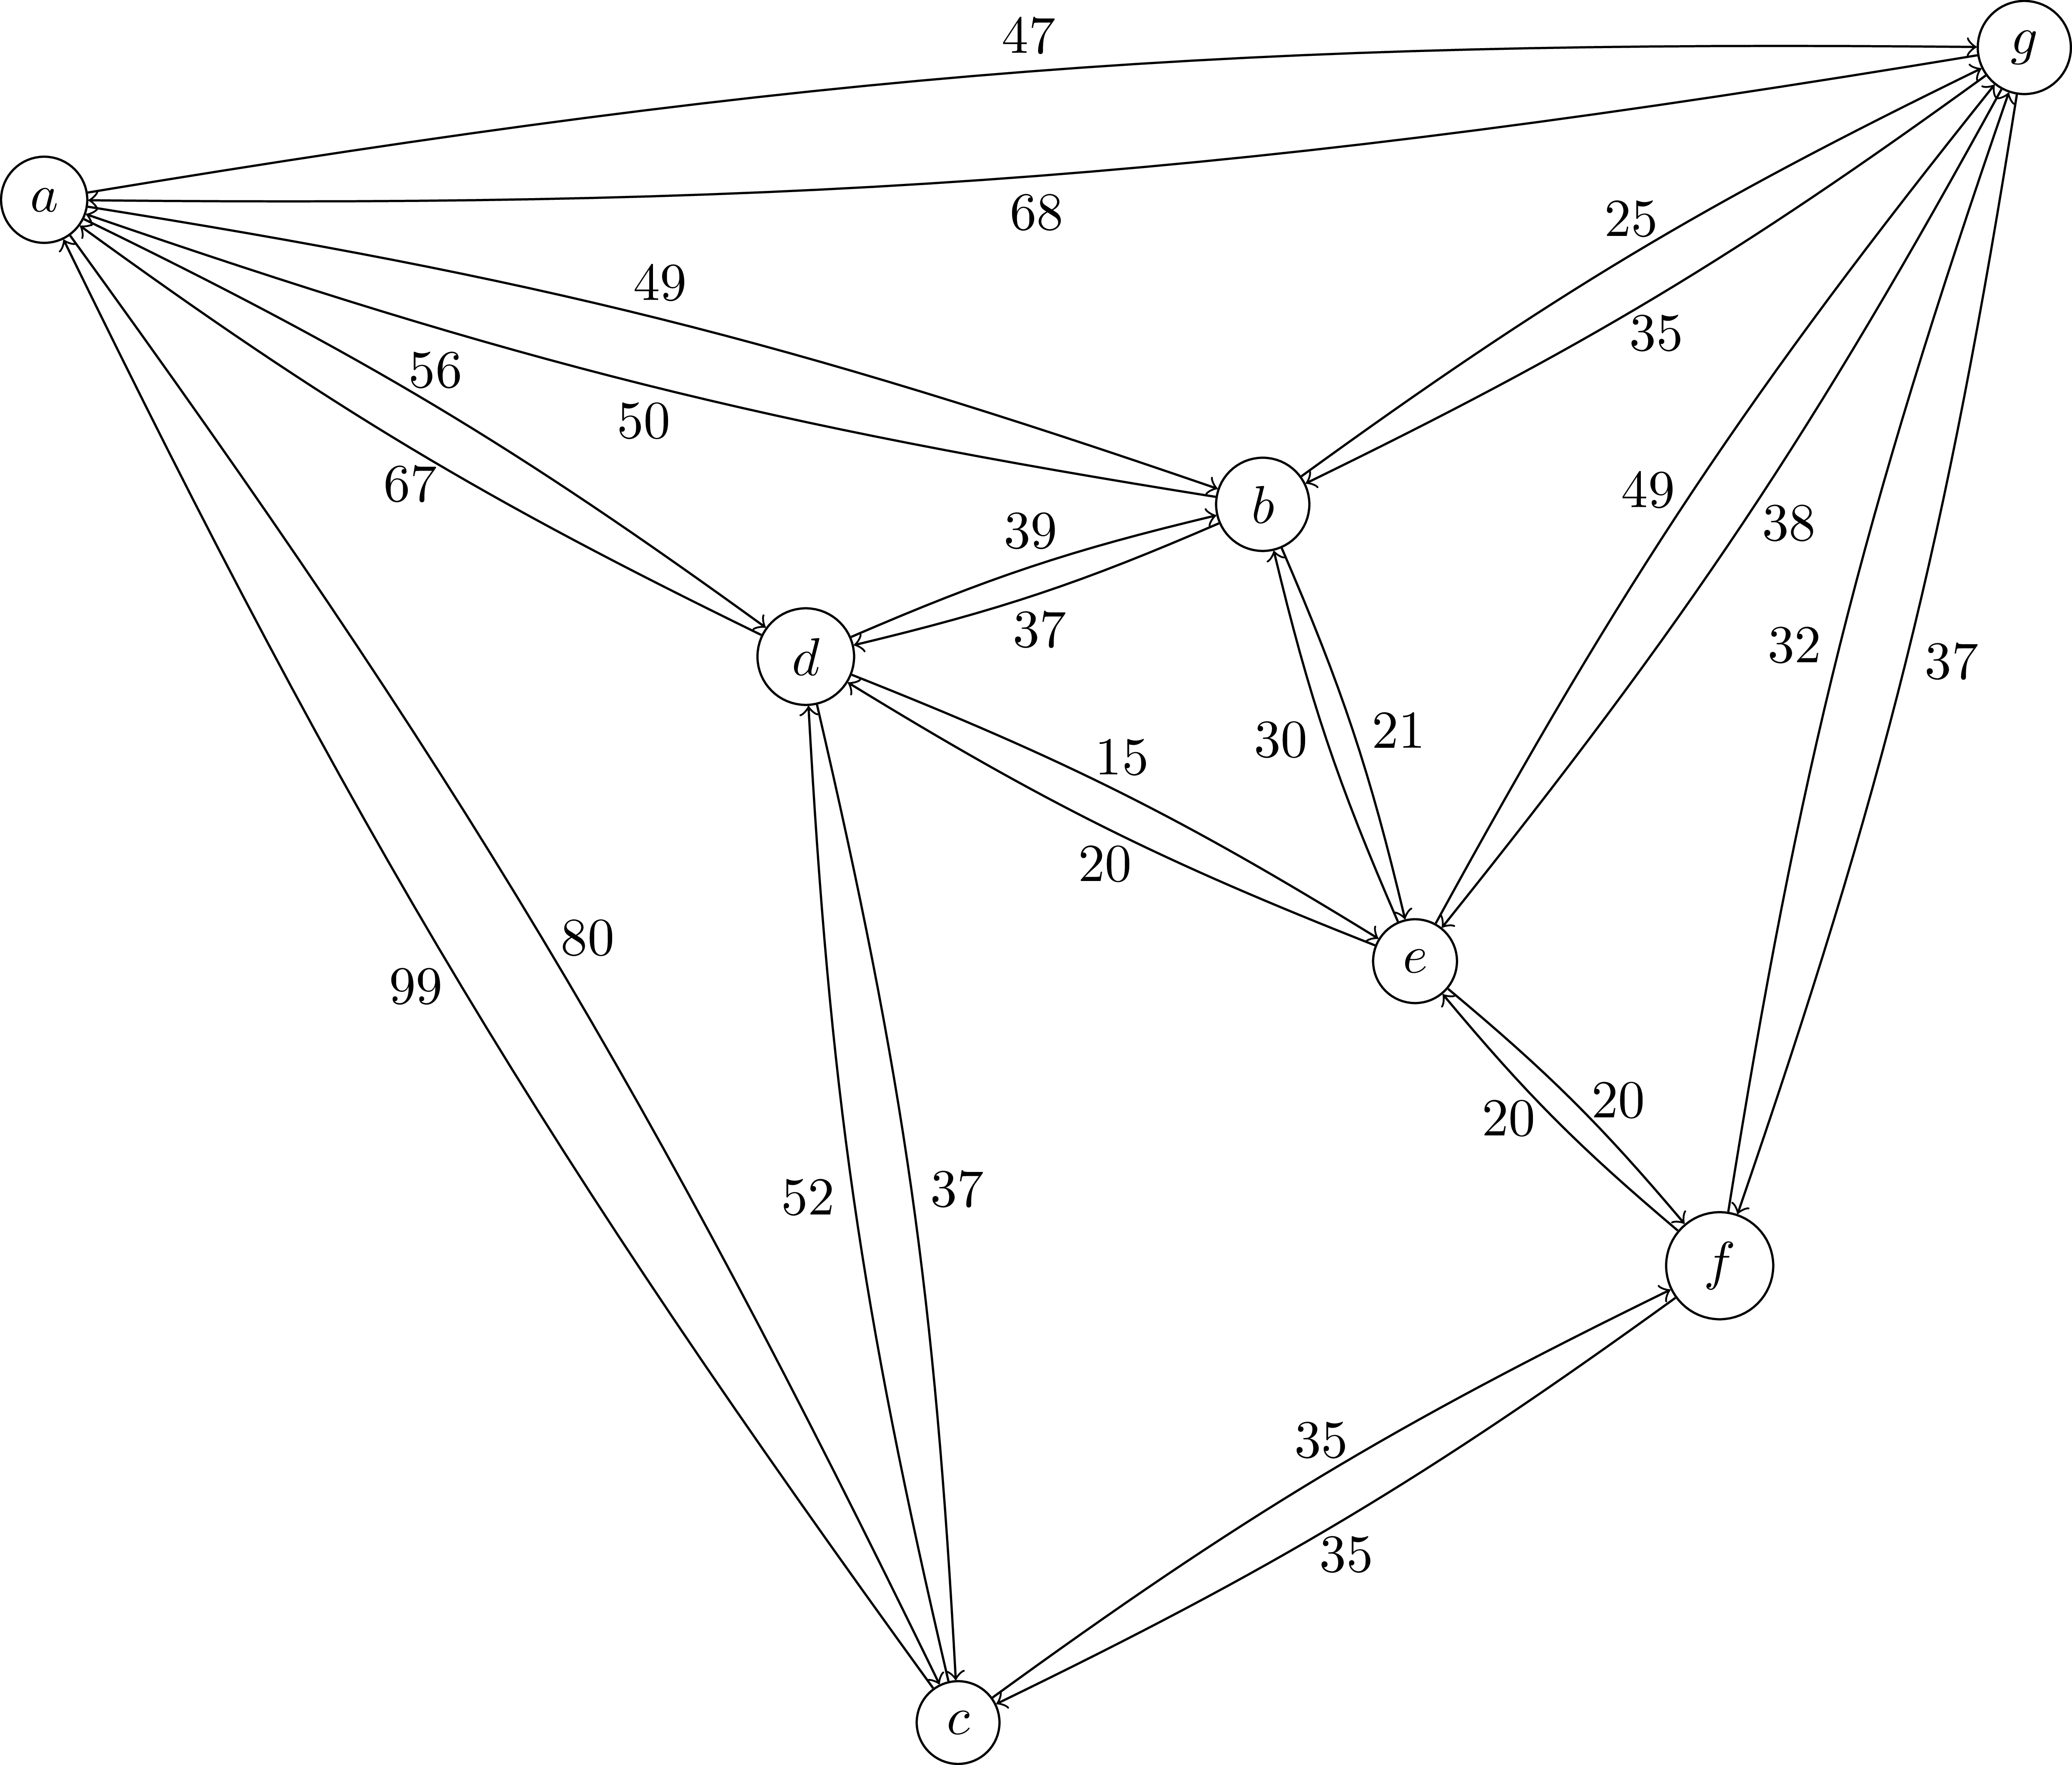
\includegraphics[scale=0.6]{/home/haroldo/dev/mip/docs/images/tspG}
		\par\end{centering}
	\caption{Grafo de distâncias de exemplo}
	
	\label{figG}
\end{figure}


\subsection{Uma Formulação Compacta}

O problema do caixeiro viajante pode ser modelado utilizando-se uma
formulação compacta, isto é, uma formulação com um número polinomial
de variáveis e restrições. Formulações desse tipo, apesar de não serem
a melhor opção de resolução em termos de desempenho para problemas
deste tipo, são convenientes para uma primeira abordagem pois podem
ser facilmente inseridas de uma vez só como entrada para um software
resolvedor. A formulação abaixo foi proposta\cite{Miller1960} nos
anos 60:

\begin{align}
\textrm{Minimize:}\nonumber \\
& \sum_{(i,j)\in A}d_{(i,j)}\ldotp x_{(i,j)}\nonumber \\
\textrm{Sujeito a:}\nonumber \\
\sum_{(i,j)\in A}x_{(i,j)} & =1\,\,\,\forall\,i\in V\label{eq:in}\\
\sum_{(i,j)\in A}x_{(i,j)} & =1\,\,\,\forall\,j\in V\label{eq:out}\\
y_{i} & \geq y_{j}-|V|+(|V|+1)x_{(i,j)}\,\,\,\forall\,(i,j)\in A:1\notin\{i,j\}\label{eq:st1}\\
y_{i} & \geq0\,\,\,\forall\,i\in V\label{eq:y}\\
x_{(i,j)} & \in\{0,1\}\,\,\,\forall\,(i,j)\in A\label{eq:x}
\end{align}

As equações \ref{eq:in} e \ref{eq:out} garantem que cada vértice
é visitado somente uma vez enquanto variáveis auxiliares $y_{i}$
são utilizadas nas equações \ref{eq:st1} para garantir que uma vez
que um arco $(i,j)$ seja selecionado, o valor de $y_{i}$ seja maior
do que o valor de $y_{j}$ em uma unidade. Essa propriedade é garantida
para todos os vértices exceto o vértice 1 que é arbitrariamente selecionado
como origem de modo a evitar a construção de sub-rotas desconectadas
como no exemplo da Figura \ref{figSub}, onde os valores das variáveis
$x_{(i,j)}$ indicados nos arcos representam uma solução viável caso
somente as restrições \ref{eq:in} e \ref{eq:out} fossem consideradas.

\begin{figure}
	\begin{centering}
		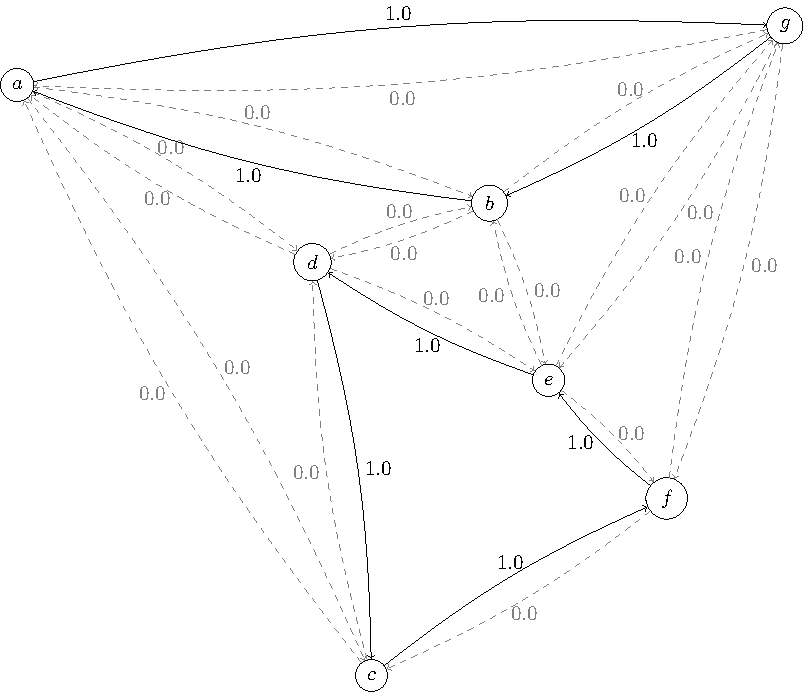
\includegraphics[scale=0.6]{/home/haroldo/dev/mip/docs/images/tspNo2Sub}
		\par\end{centering}
	\caption{Rotas desconectadas da origem}
	\label{figSub}
	
\end{figure}

A seguir temos um exemplo completo de um resolvedor em Python-MIP onde para o problema do caixeiro viajante com os dados da Figura \ref{figG}, onde o resolvedor utilizará a formulação compacta descrita anteriormente:

{\small
\begin{lstlisting}
from mip import Model, BINARY, minimize, xsum
from sys import stdout as out

N = ['a', 'b', 'c', 'd', 'e', 'f', 'g']
A = {('a', 'd'): 56, ('d', 'a'): 67, ('a', 'b'): 49, 
  ('f', 'c'): 35, ('g', 'b'): 35, ('g', 'b'): 35, ('b', 'g'): 25,
  ('a', 'c'): 80, ('c', 'a'): 99, ('e', 'f'): 20, ('f', 'e'): 20,
  ('g', 'e'): 38, ('e', 'g'): 49, ('g', 'f'): 37, ('f', 'g'): 32,
  ('b', 'e'): 21, ('e', 'b'): 30, ('a', 'g'): 47, ('g', 'a'): 68,
  ('d', 'c'): 37, ('c', 'd'): 52, ('d', 'e'): 15, ('e', 'd'): 20,
  ('d', 'b'): 39, ('b', 'd'): 37, ('c', 'f'): 35, ('b', 'a'): 50}
  
m = Model()
n, n0 = len(N), min(N)

x = { (i, j): m.add_var(var_type=BINARY, 
                        name='x(%s,%s)' % (i,j)) for (i, j) in A }
y = { i: m.add_var(name='y(%s)' % i) for i in N }

m.objective = minimize(xsum(A[a]*x[a] for a in A))

for i in N:
    m += xsum(x[a] for a in A if a[0] == i) == 1
    m += xsum(x[a] for a in A if a[1] == i) == 1
	
for (i, j) in [a for a in A if n0 not in [a[0], a[1]]]:
    m += y[i] - (n+1)*x[(i, j)] >= y[j] - n
	
m.optimize()
print('route with length {} found:'.format(m.objective_value))
out.write(n0)
nc = n0
for i in N:
    nc = [nl for nl in N if (nc, nl) in A and x[(nc,nl)].x>0.99][0]
    out.write(' -> {}'.format(nc))
\end{lstlisting}
}

Nosso grafo com a malha viária da Figura \ref{figG} é informado nas linhas 3 e 4. A estrutura de dados dicionário, disponível na linguagem Python, permite mapear convenientemente os arcos do grafo (pares ordenados) com suas respectivas distâncias. A linha 13 cria o modelo de programação linear inteira. Na linha 14 armazenamos na variável \texttt{n} o número de pontos e em \texttt{t0} o primeiro ponto da lista, que será arbitrariamente escolhido como ponto de partida de nossa rota. 

As variáveis do modelo são criadas nas linhas 16 e 17 utilizando o método \texttt{add\_var} em nosso modelo \texttt{m}. Durante a criação das restrições, será necessário referenciar as variáveis criadas. Por isso, utilizamos os dicionários \texttt{x} para mapear cada arco do grafo a sua respectiva variável binária e \texttt{y} para mapear cada nó com sua respectiva variável auxiliar contínua para eliminação de sub-rotas.

A função objetivo que minimiza a distância total dos arcos selecionados é informada na linha 19. Nesse caso, para cada arco multiplicamos sua respectiva variável binária de seleção pela distância do arco armazenada em \texttt{A}.

As restrições são criadas nas linhas 21-26. Em todos os casos utilizamos o operador \texttt{+=} sobre o modelo \texttt{m} para adicionar restrições lineares. Note que assim como na função objetivo, o somatório é efetuado com a função \texttt{xsum}. Esta função é similar a função \texttt{sum} disponível na linguagem Python mas otimizada para a situação específica de escrita de restrições lineares no pacote Python-MIP\@. O dicionário \texttt{A} que armazena as distâncias contém arcos \texttt{a} que são pares ordenados $(i,j)$=\texttt{(a[0], a[1])}. Dessa forma, a criação das restrições (1) e (2) é feita iterando-se em cada nó \texttt{i} e incluindo na linha 22 todos os arcos de saída em \texttt{i} \texttt{(a[0]==i)} em uma restrição cujo somatório das respectivas variáveis de seleção deve ser 1 e em 23 todos os arcos de entrada em \texttt{i} \texttt{(a[1]==i)} em restrições no mesmo formato.

A linha 28 dispara a otimização do modelo. Em nosso exemplo, assumimos que uma rota existe e será encontrada pelo otimizador\footnote{Em aplicações completas onde modelos de larga escala podem ser otimizados é recomendável a especificação de limites de tempo na otimização (propriedade \texttt{max\_seconds} do modelo) e a posterior checagem do sucesso do otimizador na prova da otimalidade e/ou obtenção de solução viável através da propriedade \texttt{status} do modelo.}. Desse modo, nas linhas seguintes imprimimos o custo e a sequência de visitas da rota encontrada. 

A linha 33 é um exemplo da expressividade da linguagem Python: para cada vértice criamos uma lista contendo o próximo vértice selecionado na rota ótima. Apesar de que em soluções viáveis somente haverá um vértice seguinte a cada um, a iteração pelos arcos em \texttt{A} resulta na criação de uma lista dentro dos colchetes. Essa iteração é condicional, considerando somente variáveis binárias $x$ que aparecem $=1$ na solução ótima. Como resolvedores de programação linear inteira mista utilizam computação com precisão limitada, por segurança selecionamos as variáveis com valor próximo de 1 na solução ótima. 

Os resolvedores de programação linear inteira executam uma busca em árvore onde são utilizados limites para a poda de nós. O limite superior é obtido a partir de qualquer solução viável que for encontrada durante a busca e o limite inferior corresponde ao custo obtido com a resolução do problema com as restrições de integralidade das variáveis binárias relaxadas. No nosso caso considerando domínio das variáveis $x$ como contínuo entre 0 e 1. A formulação aqui utilizada tem uma grave deficiência: o limite inferior por ela produzido é distante do custo ótimo da solução. Desse modo, a performance dos resolvedores de programação linear inteira em sua resolução é bastante pobre. 

Um desempenho muito melhor pode ser obtido com a inserção das seguintes desigualdades:

\begin{equation}
\sum_{(i,j) \in A : i\in S \land j \in S} x_{(i,j)} \leq |S|-1 \,\,\, \forall S \subset V 
\end{equation}

O problema com as desigualdades acima é que elas devem ser geradas para cada subconjunto $S$ de vértices do grafo, ou seja, para uma grafo com $n$ vértices temos $2^n-1$ subconjuntos não vazios. Inseri-las no modelo inicial é inviável exceto para instâncias pequenas. Uma solução para esse problema é o método dos planos de corte \citep{Dantzig54}, onde somente as restrições \emph{necessárias} são inseridas. O pacote Python-MIP permite uma comunicação bi-direcional com o resolvedor para que as restrições necessárias sejam inseridas durante a busca. Para isso precisamos criar uma classe que derivada da classe \texttt{ConstrsGenerator} que implemente o método \texttt{generate\_constrs}. Esse método recebe como parâmetro um modelo, onde a solução a solução corrente pode ser consultada e restrições adicionais podem ser inseridas a medida do necessário.

\subsection{Geração de Planos de Corte}

O código abaixo implementa um gerador dinâmico de restrições de eliminação de sub-rotas para nossa formulação compacta préviamente implementada.

{\small
\begin{lstlisting}
import networkx as nx

class SubTourCutGenerator(ConstrsGenerator):
    def __init__(self, Fl: List[Tuple[int, int]]):
        self.F = Fl

    def generate_constrs(self, model: Model):
        G = nx.DiGraph()
        r = [(v, v.x) for v in model.vars if v.name.startswith('x(')]
        U = [int(v.name.split('(')[1].split(',')[0]) for v, f in r]
        V = [int(v.name.split(')')[0].split(',')[1]) for v, f in r]
        cp = CutPool()
        for i in range(len(U)):
            G.add_edge(U[i], V[i], capacity=r[i][1])
        for (u, v) in F:
            if u not in U or v not in V:
                continue
            val, (S, NS) = nx.minimum_cut(G, u, v)
            if val <= 0.99:
                arcsInS = [(v, f) for i, (v, f) in enumerate(r)
                           if U[i] in S and V[i] in S]
                if sum(f for v, f in arcsInS) >= (len(S)-1)+1e-4:
                    cut = xsum(1.0*v for v, fm in arcsInS) <= len(S)-1
                    cp.add(cut)
                    if len(cp.cuts) > 256:
                        for cut in cp.cuts:
                            model += cut
                        return
        for cut in cp.cuts:
            model += cut
        return
\end{lstlisting}}

Na criação de nosso gerador de cortes informamos uma lista \texttt{Fl} de pares $(i,j)$ de vértices cuja conectividade deve ser checada em toda solução gerada. No método \texttt{generate\_constrs} consultamos as variáveis do modelo (\texttt{model.vars}) e identificamos a qual arco cada variável se refere considerando o nome das variáveis (linhas 22 e  23), utilizando o seu valor (propriedade \texttt{x}) para construção do grafo onde iremos procurar sub-rotas desconexas para geração das restrições (6). A identificação dessas sub-rotas é feita resolvendo-se o problema do corte mínimo, com o algoritmo que está disponível no pacote \texttt{networkx} (linha 18). A descoberta de sub-rotas desconexas (linhas 19) gera a restrição de restrições (cortes) que são primeiramente armazenados em um conjunto (linha 24) e posteriormente adicionadas ao modelo. Separamos esses dois passos pois restrições repetidas podem ser geradas. Na linha 25 inserimos um critério de parada para a geração dos cortes: caso um número suficientemente grande já tenha sido gerado, inserimos os mesmos no modelo e prosseguimos a otimização sem procurar por cortes adicionais. Nesse ponto convém ressaltar a função dos cortes e sua relação com o restante do modelo. Como a formulação compacta que estamos utilizando define completamente o problema, a adição de cortes é opcional, ou seja, somente feita para melhorar o desempenho do modelo. A inserção de um número muito grande de cortes por iteração pode gerar o efeito inverso que é a perda de desempenho na resolução. Para utilizamos nosso gerador de cortes com a formulação anterior basta atribuir à propriedade \texttt{cuts\_generator} um objeto da nossa classe \texttt{SubTourCutGenerator} antes da otimização do modelo.

\subsection{Integração com heurísticas}

Resolvedores de programação linear inteira iniciam o processo de resolução computando uma solução, possivelmente fracionária, obtida através da relaxação do problema. Em instâncias difíceis, a obtenção da primeira solução inteira válida pode requerer a exploração de um grande número de nós na árvore de busca. Para essas instâncias, muitas vezes uma heurística simples e rápida pode ser utilizada para geração de uma solução inicial. No pacote Python-MIP soluções iniciais podem ser facilmente informadas ao resolvedor através da propriedade \texttt{start} do modelo.
		
\bibliography{pmip-podes}
\bibliographystyle{podes-bibstyle}


\end{document}
